% THIS IS AN EXAMPLE DOCUMENT FOR VLDB 2010
% based on ACM SIGPROC-SP.TEX VERSION 2.7
% Modified by  Gerald Weber <gerald@cs.auckland.ac.nz>


% This example *does* use the .bib file (from which the .bbl file
% is produced). REMEMBER HOWEVER: After having produced the .bbl file,
% and prior to final submission, you need to 'insert'  your .bbl file into
% your source .tex file so as to provide ONE 'self-contained' source file.

\documentclass[a4paper,12pt,oneside,titlepage, fleqn]{book}
\renewcommand{\baselinestretch}{1.5}

%==============================================================
\usepackage[BoldFont, SlantFont, CJKchecksingle]{xeCJK}
\setCJKmainfont[Mapping=tex-text]{STSongti-TC-Light}
\setCJKsansfont[Mapping=tex-text]{STSongti-TC-Light}
\setCJKmonofont[Mapping=tex-text]{STSongti-TC-Light}


\usepackage[font=scriptsize,labelfont=bf]{caption}
\usepackage{wallpaper}
\usepackage{graphicx}
\usepackage{amsmath}
\usepackage{pdfpages}

% Configure your package here


%==============================================================
% page setup for NTHU thesis format
\CenterWallPaper{.30}{images/nthu-logo.pdf}

% set paper size
\special{papersize=8.5in,11in}
\topmargin=14.7mm
% \bottomargin= 14.7mm
\oddsidemargin=30mm		% left & right margin 17.45mm


% text sizes (Keep these values unchanged!)
\textwidth=150mm \textheight=240mm
\columnsep=5.0mm
\parindent=3.5mm

% misc parameters
\headsep=10mm  \headheight=0mm \footskip=18mm

% conversion to values for LaTeX
\advance\topmargin-1in\advance\oddsidemargin-1in
\evensidemargin\oddsidemargin
%==============================================================


\begin{document}
\graphicspath{{images/}}

\thispagestyle{empty}

\vspace{20mm}
\centerline{\fontsize{30pt}{\baselineskip}{國立清華大學}}
\vspace{15mm}
\centerline{\fontsize{25pt}{\baselineskip}{\underline{碩士論文}}}

\vspace{25mm}



\centerline{
\LARGE
{積體化電路設計之矽基體奈米線}
}
\vspace{10mm}

\centerline{\LARGE\textbf{
{An Integrated Circuit Design }
}}
\vspace{5mm}

\centerline{\LARGE\textbf{
for Silicon-Nanowire
}}
\vspace{50mm}

\begin{tabular}{l}
\Large{\underline{\fontsize{20pt}{\baselineskip}{系所別:電機工程學系研究所}}}
\\
\\
\Large{\underline{\fontsize{20pt}{\baselineskip}{學生姓名:103061608 張永忱}(Young-Chen Chang)}}
\\
\\
\Large{\underline{\fontsize{20pt}{\baselineskip}{指導教授:陳\hspace{5mm}新\hspace{5mm}博士}(Prof. Hsin Chen)}}
\\
\\
\\
\\
\Large{\centerline{\fontsize{20pt}{\baselineskip}{中華民國 106年3月}}}
\end{tabular}


\title{\bf \Huge An Integrated Circuit Design for Silicon-Nanowire}
\date{}
\author{
\begin{tabular}{c}
\\
\\
{\LARGE \bf Student: Young-Chen Chang}\\
{\LARGE \bf Advisor: Prof. Hsin Chen}\\
\\
\\
\\
\\
{\LARGE \bf Department of Electrical Engineering}\\
{\LARGE \bf National Tsing Hua University}\\
{\LARGE \bf Hsinchu, Taiwan, 30013, R.O.C.}\\
\\
{\large  2016}
\end{tabular}
}

% make the title area
\maketitle

%==============================================================
\frontmatter
\pagenumbering{gobble}
\thispagestyle{empty}
\chapter*{\centerline{Abstract}}
\addcontentsline{toc}{chapter}{Abstract}


Poly-silicon nanowire (SiNW) is a well-studied and interesting one-dimensional nanostructure.
Since it was introduced to the biosensor field in 2001, it has become a promising candidate for ultra-sensitive, real-time and label-free sensor device.
Nevertheless, many physical and chemical challenges constrain nanowire from being robust and practical.
Nowadays, many studies adopt the integrated-circuit techniques to solve the problems.
Circuits with different design concepts and purposes are proposed to meet practical needs.

In this thesis, based on the nanowire designed by Prof.Yang (National Chiao Tong University), we design our own read-out circuit.
This research first analyzes biological experiments results (From Prof.Yang) and the electrical characteristics of the nanowires.
The circuit specification and design is then based on these data analysis.

The circuit is capable of performing both DC-sweep ($I_D$-$V_G$ sweep) and transient measurement.
Moreover, we proposed a measurement method a combining of these two functions.
We believe this method mitigates the device variability induced by the fabrication process.
Currently, most operations in this method are manual.
We hope to make them automatic in the future by inducing digital circuits and constructing a system-level structure.






\thispagestyle{empty}
\chapter*{\centerline{\fontsize{16pt}{\baselineskip}{中 \quad 文 \quad 摘 \quad 要}}}
\addcontentsline{toc}{chapter}{中文摘要}
\fontsize{14pt}{\baselineskip}

\quad 矽基體奈米線(以下簡稱奈米線)乃ㄧ有趣並經過充分研究的一維奈米結構物。
自從於 2001 年該元件被引入生物量測領域,奈米線就被賦予高度期望,能成為具有高靈敏度、即時性和不需生物標記等優勢的生物分子感測元件。
雖然如此,目前仍有有物性和化性上的因素,限制了奈米線的良率和實用性。
如今,許多研究採用了積體電路的技術,設計出在概念上和目的上不同的電路,來解決奈米線所遇到的問題和應付特定的需求。

我們使用由交大楊裕雄老師的奈米線元件和一部分量測資料,設計出一套元件訊號讀取電路。
本篇研究首先進行生物實驗和電性量測的數據分析,接著根據分析結果來訂出電路的規格和進行電路設計。

我們的電路可以進行直流掃描量測(DC-sweep)和暫態量測(Transient measurement)。
並且,藉由結合此二量測,我們提出一套元件量測方式。
這個量測方式被認為具有減輕因製程變異性而導致的元件差異問題(Device Variability)的能力。
目前,該量測方式多採用手動操作,我們希望日後能引入數位電路於系統性架構,使量測能夠自動化。


\clearpage % To prevent the page number missing
\setcounter{tocdepth}{4}
\setcounter{secnumdepth}{4}
\tableofcontents
\listoffigures

\mainmatter
\pagenumbering{arabic}
\chapter{Introduction}
\section{Motivation}
Poly-silicon nanowire(SiNW) is a well-studied and promising one-dimensional nanostructure.
It was first introduced to the biosensor field in 2001\cite{C2001} and has become a potential candidate for various features such as high surface-to-volume ratio, ultra sensitivity, label-free electrical detection and real-time measurement.

Although there have been substantial advances on nanowire structure design \cite{R1}, the work on the systems-level engineering is still insufficient.
Systems designed for a specific purpose can help the device to meet practical needs such as noise reduction, real-time measurement, and analog-to-digital conversion.
Moreover, there are still several challenges that may be overcome through a better signal acquisition system \cite{R1}.

One of the challenges is that the mass production of robust nanowire device is still improbable.
Device disparity may be the main reason among others.
This problem also happens to the measurement of our nanowire (Fig.~\ref{fig:disparity}).
The nanowire we use is made by Professor Yang's team (National Chiao Tong University).
And according to them, the nanowire uses thick gate dielectric and have non-regular cross-sectional shape, which results in the problem of fabrication uncertainty \cite{C6}.


\section{Design Overview}
In this project, we design a nanowire read-out circuit with two modes: DC Sweep mode and Transient Measurement mode.
In the DC Sweep mode, one can use the circuit to perform a DC sweep of drain-to-source current ($I_D$) to show how the gate voltage ($V_G$) changes, or gives nanowire a constant $I_D$ and measures the $V_{G}$ response to different solution concentration.
In the Transient Measurement mode, the circuit detects and amplifies the variance of drain current ($I_D$) with constant bias voltages applied ($V_D$, $V_G$, $V_S$).
We also combine two modes to implement a proposed method that may mitigate the disparity problem.

\subsection*{Dealing with the Disparity Problem} \label{section:twqAssumption}
The proposed method base on two assumptions:
\begin{enumerate}
    \item The nanowire transconductance ($g_m = \frac{\partial I_D}{\partial V_{GS}}$) depends on $I_D$ and independent on $V_{GS}$.
    \item The concentration difference of biomolecule can be viewed as a voltage signal input to the gate end of a transistor.
\end{enumerate}
The first assumption implies one can control the nanowire transconductance by its $I_D$.
The second assumption means that as long as different nanowire elements have the same transconductance, the output current induced by a concentration difference should be same.

The method works as follows:

\paragraph*{Initial stage}
At the beginning of each measurement event, we perform a DC sweep with the DC Sweep mode.
By analyzing the sweep results with numerical method, we keep all nanowire devices under a selected transconductance by controlling their $I_D$ and corresponding $V_G$.

\paragraph*{Measurement stage}
We bias the circuit in the Transient Measurement mode at this stage.
Since the transconductance of all devices are same, they should behave uniformly based on assumption 2.
At the end of the stage, we return to the DC Sweep mode to reset $I_D$ of the elements.
The circuit adjusts their $V_G$ to do so.

At the beginning of each measurement stage, a device always has the same $I_D$ but different $V_G$.
Based on assumption 1, its transconductance is kept constant.


The other details are reviewed in chapter 5.
Currently, most operations are manual.
We hope to make them automatic in the future, which may require digital circuits.

\section{Design Flow and Chapter Layout}
In this thesis, there are six chapters sorted according to the design flow.

Chapter 2 reviews the basic theories and the literature that are related to our work.
Most of those are the drain current of nanowire sweeping along the gate voltage (Id-Vg curves).
We present some of the raw data and the analysis results in this part.

Chapter 3 gives a brief description of nanowire structure.
It is then followed by two sections about some measurement and data analysis.
The data of the first one is from the biological experiments while the second one is from the electrical measurement.
We use the analysis results to design the read-out circuit.

Chapter 4 is an ``accessory''.
This chapter contains the discrete circuit which was designed for ion-sensitive field-effect transistor (ISFET) \cite{SF1}.
We construct it and perform some electrical measurement.
The purpose of this process is to practice the constant-current constant-voltage method.
The outcomes are deficient, and it is its reference value which we spotlight.

Chapter 5 talks about the schematic, design process and the simulation results of the read-out circuit.

Chapter 6 presents the measurement results of our integrated circuit and the conclusion of this project.





% This circuit has two operation mode.
% One is the ``Gate Voltage Tracing (GVT)" mode, and the other is the ``Current Variance Measure (CVM)" mode.



%
% {\color{red}A better measure method}
%
%  The concentration changing of the testing solution effect the intrinsic characteristics of nanowire.
% There are a variety of method for quantifying the affect.
% The most common ones are finding drain-source current and nanowire drain-to-source resistance.
% The method that Yang's team employed is to find several Id-Vg sweeping curves and see the rising/falling trend of them (Fig.~\ref{fig:IdVgandgbsId} (a)).
%  By the method of Yang's team, we had an intuition using transconductance instead of drain-to-source resistance may give a more {\color{red}usful} result.
% {\color{red}Because the }
%
%
% In the beginning, we adopted Yang's method and made some modification to it.
% By finding the derivative of Id with respect to Vg, we have the relation between Id and transconductance of nanowire (Fig.~\ref{fig:IdVgandgbsId} (b)).

% In our biosensor system, nanowire is treated as a MOSFET.
% Its gate bias under a specific voltage source
% And the bio-signal is viewed as small voltage signal input to the gate.
%
%
%  with its drain-source current ($I_{ds}$)  biased by a pmos current source.
% When a measurement event happens (such as a DNA concentration variation), the transconductance of nanowire changes and induces a current variance.
% This variance is converted into an amplified voltage signal.
% After the measurement, a feedback circuit pulls up/down the nanowire gate-source voltage ($V_{gs}$) to set $I_{ds}$ to the initail value.




%
% The different concentration of the measuring solution induce the change of nanowire transcconduction.
% By keeping bias voltage (drain, source, gates) same, the transconduction chage directly effect the drain-source current.
% The current variance signal is converted into voltage signal and is amplified.
% After each measurement, the drain-source current of nanowire returns to the constant value by a feedback circuit, which adjusts the gate-source voltage.
% the current variance induced by the difference of the solution concentration
% The other is the process variation. Since




\chapter{Literature Review \&}
As previously mentioned in the introduction section, the read-out circuit we proposed has two operation mode (DC and AC).
The DC mode is for drain current biasing while the AC mode is for current variance measurement.
Each of them references different sources.

\section{DC Sweep and Source Follower}
In this section, we review the knowledge and an article that is related to our design of large signal mode (DC).

\subsection{Constant Current}


\subsection{Source Follower}
{\color{red}{Fig of source follower}}
As one of the basic single stage amplifier, source follower (common drain) are employed to transfer voltage signal from gate to source while keeping drain current constant.
The transfer function can be derived as:
\setlength{\mathindent}{6.5cm}
\begin{align}
    \frac{V_{out}}{V_{in}} & = \frac{r_{ds}g_m}{1 + r_{ds}g_m} \\    \label{eq:sfTF}
                           & \approx 1 \qquad \text{ for } \quad r_{ds}g_m >> 1
\end{align}
$g_m$ is the transconductance ($\frac{\partial I_d}{\partial V_{gs}}$) and $r_{ds}$ is the drain-to-source impedance.
Although we haven't seen it is applied to nanowire, there have been several applications in the read-out circuits of ISFET (Ion-sensitive Field-effect Transistor)\cite{SF1, SF2} for a long time.

In ``Rapid Detection of E.coli Bacteria using Potassium-Sensitive FETs in CMOS", ISFET is applied as a biological transducer that convert detected bio-signal into it's input signal on the gate-end, which is resemble to our biosensor of nanowire.
An read-out circuit of source follower is served as the analog front-end.
The bio-signal induced voltage difference at the ISFET gate-end are converted to the source-end.
There is no need for an extra current-to-voltage converter which may import more signal fluctuation such as shot noise or flicker noise.
But on the other hand, the circuit requires a biasing current source.
This current source may have to be stable, noiseless or wide-range on demand.
And since the current value are usually under micro-scale even nano-scale, it is impractical to merely use external current source.
The article use two resistors and an op-amp to design a current scale down circuit.
Bias current decreases in proportional to the resistance ratio (N) of one resistor to another.
Moreover, by keeping Vds at a constant value (0.5v), the circuit also removes {\color{red}the channel affect which is a factor that may effect linearity of the results.}
It is showed in the schematic below that two op-amp based unit gain buffer are added to force the voltage at drain-end follows the source-end.

{\color{red} Schematic}

An issue need to be noticed is the impedance matching between the element and the current source circuit.
It is known that the output impedance of current source should be much larger than the input impedance of the biased element.
The equation for the output impedance of source follower is:

\begin{align}
    & \frac{r_{ds}}{1 + g_mr_{ds}}\\
\intertext{This equation can be simplified as:}
    & \frac{1}{g_m} \qquad \text{ for } \quad g_mr_{ds} >> 1 \label{eq:rsf2}
\end{align}
We also compute the output impedance of the current source circuit:
\begin{equation} \label{eq:rcs}
    N\times R_i
\end{equation}
$R_i$ is the impedance of the current source {\color{red}{I1 in Fig}}.
In the integrated circuit, $R_i$ is not ideal but usually close to the $r_{ds}$ of a single MOSFET.

As mentioned, Eq.\ref{eq:rcs} should be far larger than Eq.\ref{eq:rsf2}.
However, $g_m$ is proportional to the $I_d$, which means Eq.\ref{eq:rsf2} is inversely proportional to N.
When the bias current decreases, the output impedance decreases while the input impedance at the ISFET source-end increases.
This creates a lower boundary of the bias current.

The source follower structure provides a direct signal transition method.
It is a good candidate for the read-out circuit with the aim of detecting transconductance or threshold voltage variance.
Nevertheless, post-processing such as amplification and filtering are necessary.
The experiment results in the article are untreated.
Some strong signal attenuation exist, which are mainly caused by low-frequency noise and ISFET drift \cite{Drift}.
The drift problem are dealt with through some signal processing techniques while noise problems are left untreated.

We constructed this circuit with discrete elements and applied it to our nanowire. The results are presented in chapter 4.


\section{Small Signal (AC) Measurement Method Review}
In previous section, the source follower we mentioned exhibited compelling advantages as a signal processing structure of nano-device.
However, the structure overcomes obstacles when being applied to the small signal detection.
Parasitic capacitors and resistors can severely influence the results.
We take a simple MOSFET for example.

{\color{red}{Fig of parasitic mosfet}}

With the parasitic elements from the figure above are included, we modified the transfer function Eq.\ref{eq:sfTF}
\begin{align}
    \frac{r_{ds}(sC_{gs} + gm)}{1 + r_{ds}(gm + s(C_{gs}+C_s))}
\end{align}
The equation can be similar to Eq.\ref{eq:sfTF} which roughly equals to 1 as long as $C_s$ is far more smaller than $C_{gs}$.
Unfortunately, $C_s$ can be large since the output end of source follower usually connects to the next stage input or even the chip pad.
In that case, the parasitic capacitors may attenuate the signal as signal frequency increase.

Parasitic element is an issue and deserve more consideration.
{\color{red}Works} we present below combine capacitance measurement with nanowire measure.   %not sure how many works yet.


The measurement system for ZnO-nanowire based sensor array from \cite{Juv1} applies the Time-over-Threshold techniques to its read-out circuit (Fig.\ref{fig:tot1}).
The circuit alternatively charges an on-chip capacitor ($C_{int}$) with a constant current and discharges it through the nano-material resistance (nanowire).
An inverter with its output switches from on to off when the capacitor is charged to its input threshold voltage, and vice versa.
This behavior convert information of nanowire such as capacitance and resistance into time information.
Both $C_{int}$ and capacitance of nanowire ($C_{NW}$) (from drain to source) effect charging time and together with the drain-to-source resistance effect the discharging time.

The work presented in \cite{Juv1} doesn't have enough explanation about how do they interpret the capacitance and resistance information.
It simply mentioned that a microcontroller is responsible for these calculation.
Besides, the work lacks simulation and experiment of using complex elements as measure target.
Most of the results are measurement of using concrete resistor as the substitute for nanowire and regard the $C_{NW}$ as 0p.
The only nanowire experiment given at last doesn't has good performance.

The recent publicans \cite{Juv2} by the team is more elaborate.
In Fig.\ref{fig:tot2}, nanowire append between point A and B.
The charing current is able to be applied from Mp1 or Mp2, which is determined by the ``sel" signal with the aid from the MUXs.
This is simply mean to perform a reverse measurement and we ignore it by assume sel = 1 and point B is virtually ground.
Now, we can see that the circuit design concept is actually same.
The current charge both $C_{int}$ and $C_{NW}$.
When the voltage at A exceed the threshold voltage, the output switches to off and feedback to turn off the Mp1.
(To be noted that the inverter at the output satge in \cite{Juv1} is replaced by a schmitt trigger.)
Then the capacitor discharges through nanowire ($r_{ds}$).
The right-bottom plot in Fig.\ref{fig:tot2} defines $T_0$ as the charging time and $T_1$ as the discharging time.
The derivation of the $R_{NW}$ and $C_{NW}$ in the work can be simplified as:
\setlength{\mathindent}{2cm}
\begin{align}
                         C_{NW}            & = T_0 - C_{base}\\
                         R_{NW}            & = \frac{T_1R_{par}}{(C_{NW} + C_{base})R_{par} - T_1}\\
    \text{where} \qquad  R_{NW} || R_{par} & = \frac{T_1}{C_{NW} + C_{base}}
\end{align}
$C_{base}$ are the $C_{int}$ plus parasitic capacitance and $R_{par}$ the parasitic resistance.
These parasitic elements comes from the transistor in the integrated circuit block such as MUX and Mp.
It must be noted that we doesn't concern the hysteresis of the schmitt trigger here owing to simplicity.











\begin{figure}[!htbp]
    \centering
    {\fontfamily{pag}\selectfont\textbf{
        \def\svgwidth{5.0cm}
        \fontsize{6}{7}\selectfont
        \input {images/drawing-1.pdf_tex}
    }}
    \fontsize{6}{7}\selectfont
    \caption{Nanowire Structure}
    \label{fig:tot1}
\end{figure}
\begin{figure}[!htbp]
    \centering
    {\fontfamily{pag}\selectfont\textbf{
        \def\svgwidth{5.0cm}
        \fontsize{6}{7}\selectfont
        \input {images/drawing-1.pdf_tex}
    }}
    \fontsize{6}{7}\selectfont
    \caption{Nanowire Structure}
    \label{fig:tot2}
\end{figure}
 % detects and calculates both resistance and capacitance of ZnO-nanowire based sensor array through a read-out circuit and an external microcontroller.






\section{Data Analysis}

\chapter{Nanowire Structure and Measurement}
In this chapter, we present the experiment data and some analysis which are the foundation of our circuit design.
The first section gives a brief description of our silicon nanowire element.
The second section provides the data of the biology experiments.
The last section presents the data of the electrical measurement, on which our circuit design spec depends.

\section{Brief Description of Nanowire Structure}
The nanowire we use is made by Prof.Yang's team (National Chiao Tong University)\cite{C5}.
Fig.\ref{fig:drawing} is the sectional view of the nanowire structure.
The fabrication process is based on the poly-silicon sidewall spacer technique.
The n-Type doped poly-SiNW FET has 2 to 10 poly-silicon channels.
Each channel is 80nm in width and 2µm in length.
A Large portion of the channel surface is exposed to environment.
The exposed region, through several post-process, capture the DNA probe and serve as the sensing site for DNA molecules.\cite{C5, C6}

\begin{figure}[!htbp]
    \centering
    {\fontfamily{pag}\selectfont\textbf{
        \def\svgwidth{5.0cm}
        \fontsize{6}{7}\selectfont
        \input {images/drawing.pdf_tex}
    }}
    \fontsize{6}{7}\selectfont
    \caption{Nanowire Structure}
    \label{fig:drawing}
\end{figure}


\section{Biology Experiment}
The biology experiment data are provided by Prof.Yang's team.
These data are the Id-Vg measurement of the same biomolecule placed under different circumstances or with different nanowire elements.
With each measurement repeated three times, we find the mean and standard deviation (SD) of them and consider the SD value as the intrinsic noise of nanowire.
We want to ensure that such noise should not be greater than the signal.
To be more specific, we examine whether the Id-Vg curves of different concentration overlap with each other or not.
We present an example below:

\begin{figure}[!htbp]
    \centering
    \begin{minipage}[t]{0.4\textwidth}
        \centering
        \includegraphics[scale=0.3]{images/chapter3/208_devices/L2-8_log.png}
        (a)
    \end{minipage}
    \hfill
    \begin{minipage}[t]{0.4\textwidth}
        \centering
        \includegraphics[scale=0.3]{images/chapter3/208_devices/L2-10_log.png}
        (b)
    \end{minipage}
    \caption{Concentration-dependent $I_D$-$V_G$ curves of two equivalent nanowire elements.
    In (a), the measurement result of 1fM and 100fM biomolecule solution is distinguishable. There is no overlap between two curves. This is not true in (b).}
    \label{fig:SD_sucandfail}
\end{figure}

The Fig.\ref{fig:SD_sucandfail} are concentration-dependent measurements (1 femto mole(fM) and 100fM biomolecule solution) obtained with two elements ((a) and (b)).
The two curves in the (a) are distinguishable from the other after gate voltage of 1.4v
They are not distinguishable in the (b) since they overlap each other.
We thus assert that the element of (b) can't detect the concentration difference between 1fM and 100fM.
The noise is stronger than the signal (The signal means the $I_D$ difference caused by the concentration difference).
The element of (a) can do so if it is biased at gate voltage larger than 1.4v or drain current larger than 1E-11.

\begin{figure}[!htbp]
        \includegraphics[width=1\textwidth]{images/chapter3/128_allT_mag.png}
    \caption{Concentration-dependent $I_D$-$V_G$ curves.
    Since the biomolecule is negative-charged, the lower the concentration is, the higher the curve is.
    To be noticed, the 10fM curve is closer to the curve of 1pM than 100aM.
     }
    \label{fig:SD_allT}
\end{figure}

In Fig.\ref{fig:SD_allT}, $I_D$ increase with the biomolecule concentration.
One can find that there is only a few ``space'' between PBS buffer and solution containing biomolecule with the concentration of 100aM.
Hence the 100aM should be the limit of detection.

It is worth noting that there is more space between 100aM and 10fM than the space between 10fM and 1pM.
And the noise rate: ${SD} / {Mean}$ is independent of concentration (Fig.\ref{fig:SD_allT2}).
Hence we say that the ``resolution'' for detecting concentration ranging from 100aM to 10fM may be better than the that ranging from 10fM to 1pM.
\begin{figure}[!htbp]
        \includegraphics[width=1\textwidth]{images/chapter3/128_allT_error.png}
    \caption{The noise rate of Fig.\ref{fig:SD_allT}. The noise rate is obtained by dividing SD by Mean.}
    \label{fig:SD_allT2}
\end{figure}

\subsection*{Appropriate operation region} \label{section:biasVg}
In \cite{C6}, the team found that ``the induced change of current ($I_D$) following biomolecule was dependent on the applied gate voltage (VG)'' (Fig.).
In other words, a ``biomolecule concentration resolution'' seems to depend on $V_G$
The team tried to find a bias gate voltage range which can induce more current response.
In our opinion, the induced change of current ($I_D$) following biomolecule is not directly dependent on $V_G$.
Based on the our assumption 2 (section\ref{section:twqAssumption}), it depends on the transconductance.
The phenomenon is found by $I_D$-$V_G$ curves, which means the $V_G$ also affect the $I_D$ which cause different transconductance.

Furthermore, we think the noise effect should be taken into consideration.
Some kinds of noise have  positive correlations with transconductance.

Still, we want find an appropriate operation region of nanowire that has the largest concentration resolution.
We proposed a comprehensive method that one should choose the operation region with more ``noise tolerance''.
The noise tolerance is defined as:
\setlength{\mathindent}{2cm}
\begin{align}
    noise \quad tolerance = \frac{I_D1 - SD1 - (I_D2 + SD2)}{I_D2}
\end{align}
$I_D$ and $SD$ are the mean and standard deviation of a curve.
The larger the noise tolerance implies there is more space between two curves.
And more space implies the less chance of overlapping between to concentration curves may happens.

We present analysis results from three nanowire elements.
The Fig.\ref{fig:SD_Device}(a), (c), (e) are the $I_D$-$V_G$ curves of three elements and the Fig.\ref{fig:SD_Device}(b), (d), (f) are the noise tolerance respectively.
One can observe in (b) and (d) that there is first a rising trend then followed by a drop as gate voltage decrease.
The drop doesn't exist in (f) may because the weak inversion is too narrow.
The transistor enters into the reverse region before the drop appears.
The highest points of (b) and (d) locate in the weak inversion region and is close to the transition region (The region between strong inversion and weak inversion region).
We therefore suggest that in this section nanowire should has the largest concentration resolution.


\begin{figure}[!hbtp]
    \centering
    \begin{minipage}[t][20cm][t]{1\textwidth}
        \begin{minipage}[t]{0.3\textwidth}
            \centering
            \includegraphics[width=1.8\textwidth]{images/chapter3/208_devices/L2-7_log.png}
            (a)
        \end{minipage}
        \hfill
        \begin{minipage}[t]{0.3\textwidth}
            \centering
            \includegraphics[width=1.6\textwidth]{images/chapter3/208_devices/L2-7_margin.png}
            (b)
        \end{minipage}
        \vfill
        \begin{minipage}[t]{0.3\textwidth}
            \centering
            \includegraphics[width=1.8\textwidth]{images/chapter3/208_devices/L2-8_log.png}
            (c)
        \end{minipage}
        \hfill
        \begin{minipage}[t]{0.3\textwidth}
            \centering
            \includegraphics[width=1.6\textwidth]{images/chapter3/208_devices/L2-8_margin.png}
            (d)
        \end{minipage}
        \vfill
        \begin{minipage}[t]{0.3\textwidth}
            \centering
            \includegraphics[width=1.8\textwidth]{images/chapter3/208_devices/L2-12_log.png}
            (e)
        \end{minipage}
        \hfill
        \begin{minipage}[t]{0.3\textwidth}
            \centering
            \includegraphics[width=1.6\textwidth]{images/chapter3/208_devices/L2-12_margin.png}
            (f)
        \end{minipage}

    \end{minipage}
    \caption{}
    \label{fig:SD_Device}
\end{figure}



\section{Electrical Measurements}
This section presents the data analysis results.
The data are obtained from our measurements with the source meter (Keithley 2602).
To exclude the ion effect, we placed nanowire elements in dd-water instead of biomolecule solution.
And their poly-silicon channel surfaces are only processed with {\color{red}OH ions.}

\subsection{Front Gate and Back Gate}
Our nanowire has two gates available: floating gate (liquid gate) and back-gate.
We choose floating gate as the operation gate mainly because the floating gate can induce larger drain-current.
In other words, it has higher transconductance (Fig.\ref{fig:IdVgandgbsId}).
In our circuit design, nanowire is placed in a feedback loop where its transconductance is proportional to the loop gain (chapter 5).

\begin{figure}[!htbp]
    \centering
    \begin{minipage}[t][0.1\textheight]{0.4\textheight}
        \centering
        \def\svgwidth{14cm}
        \fontsize{6}{15}\selectfont
        \input {images/FgBg_Compare_Id.pdf_tex}
        (a)
    \end{minipage}
    \hfill
    \begin{minipage}[t][0.1\textheight]{0.4\textheight}
        \centering
        \def\svgwidth{14cm}
        \fontsize{6}{15}\selectfont
        \input {images/FgBg_Compare_Id_dev.pdf_tex}
        (b)
    \end{minipage}
    \caption{Comparison between the DC sweep of voltage on the floating gate and back gate. (a) $I_D$ (b) Transconductance ($g_m$): the derivative of $I_D$}. The traansconductance of the floating gate is larger than the back gate.
    \label{fig:IdVgandgbsId}
\end{figure}


There are some advantages of back-gate.
One of them is the ability to lower the 1/f noise \cite{C7, C8}.
However, this only happens in a very high gate voltage, which is not practical in the integrated circuit design.

\subsection{Transconductance}
The most crucial parameter for our circuit design is the transconductance ($g_m$).
We acquire it by finding the partial derivative of $I_D$ of $V_{G}$.
Since in section.\ref{section:IdGm} we proved that $g_m$ is related to $I_D$, we plot the $g_m$-$I_D$ curve to reveal their relation (Fig.\ref{fig:pIdVg}(b)).

\begin{figure}[!htbp]
    \centering
    \begin{minipage}[t][0.1\textheight]{1\textwidth}
        \centering
        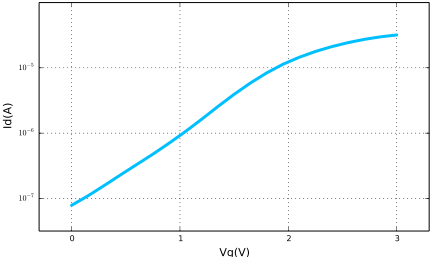
\includegraphics[width=0.6\textwidth,natwidth=610,natheight=442]{images/pIdVg.png}
        (a)
    \end{minipage}
    \hfill
    \begin{minipage}[t][0.1\textheight]{1\textwidth}
        \centering
        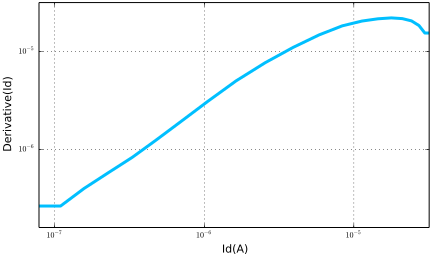
\includegraphics[width=0.6\textwidth,natwidth=610,natheight=442]{images/pIdgbs.png}
        (b)
    \end{minipage}
    \caption{Eelectrical response of a nanowire element. (a) Sweep $V_G$ and measure the $I_D$ changes. And by finding the transconductance ($g_m$): the derivative of $I_D$ of $V_G$, we plot (b) the $g_m$-$I_D$ curve}
    \label{fig:pIdVg}
\end{figure}

The $g_m$-$I_D$ plot indicates that there is a ``linear region'' where $g_m$ is proportional to $I_D$.
This corresponds to our induction (Eq.\ref{eq:gm_weak}).
We can recognize that our nanowire element is operated in weak inversion region when $I_D$ is less than 10$\mu$A.
Therefore, by the section.\ref{section:biasVg}, we decide our the $I_D$ of our nanowire should be operated below 10$\mu$A.

We also proved that the transconductance under this region is unaffected by the $V_{DS}$.

\begin{figure}[!htbp]
    \centering
    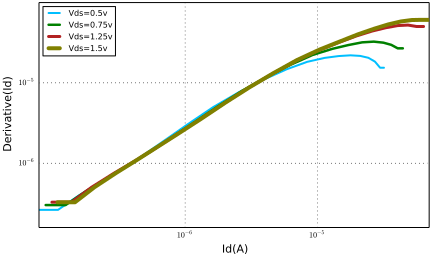
\includegraphics[width=0.8\textwidth]{images/pIdgbs_Vd.png}
    \caption{Id-transconductance with Vds variance}
    \label{fig:Idgbs_Vd}
\end{figure}

\subsection{Drain-to-source impedance ($r_{ds}$)}
In our circuit design, we keep $V_{DS}$ constant.
By the measurement in last section, 0.7 is enough to keep nanowire in saturation region for $V_G$ range from 0v to 3v.
However, due to the fabrication variance, the value varies from 0.75v to 1v.

We concern about how the $I_D$ effect $r_{ds}$.
The way we obtained $r_{ds}$ is as follows:
\begin{enumerate}
    \item Perform $I_D$-$V_G$ sweep with two different $V_D$.
    \item Find the difference of $I_D$ at each $V_G$ sweep point and divide it by the difference of $V_D$.
\end{enumerate}
The result is as Fig.\ref{fig:rds}

\begin{figure}[!htbp]
    \centering
    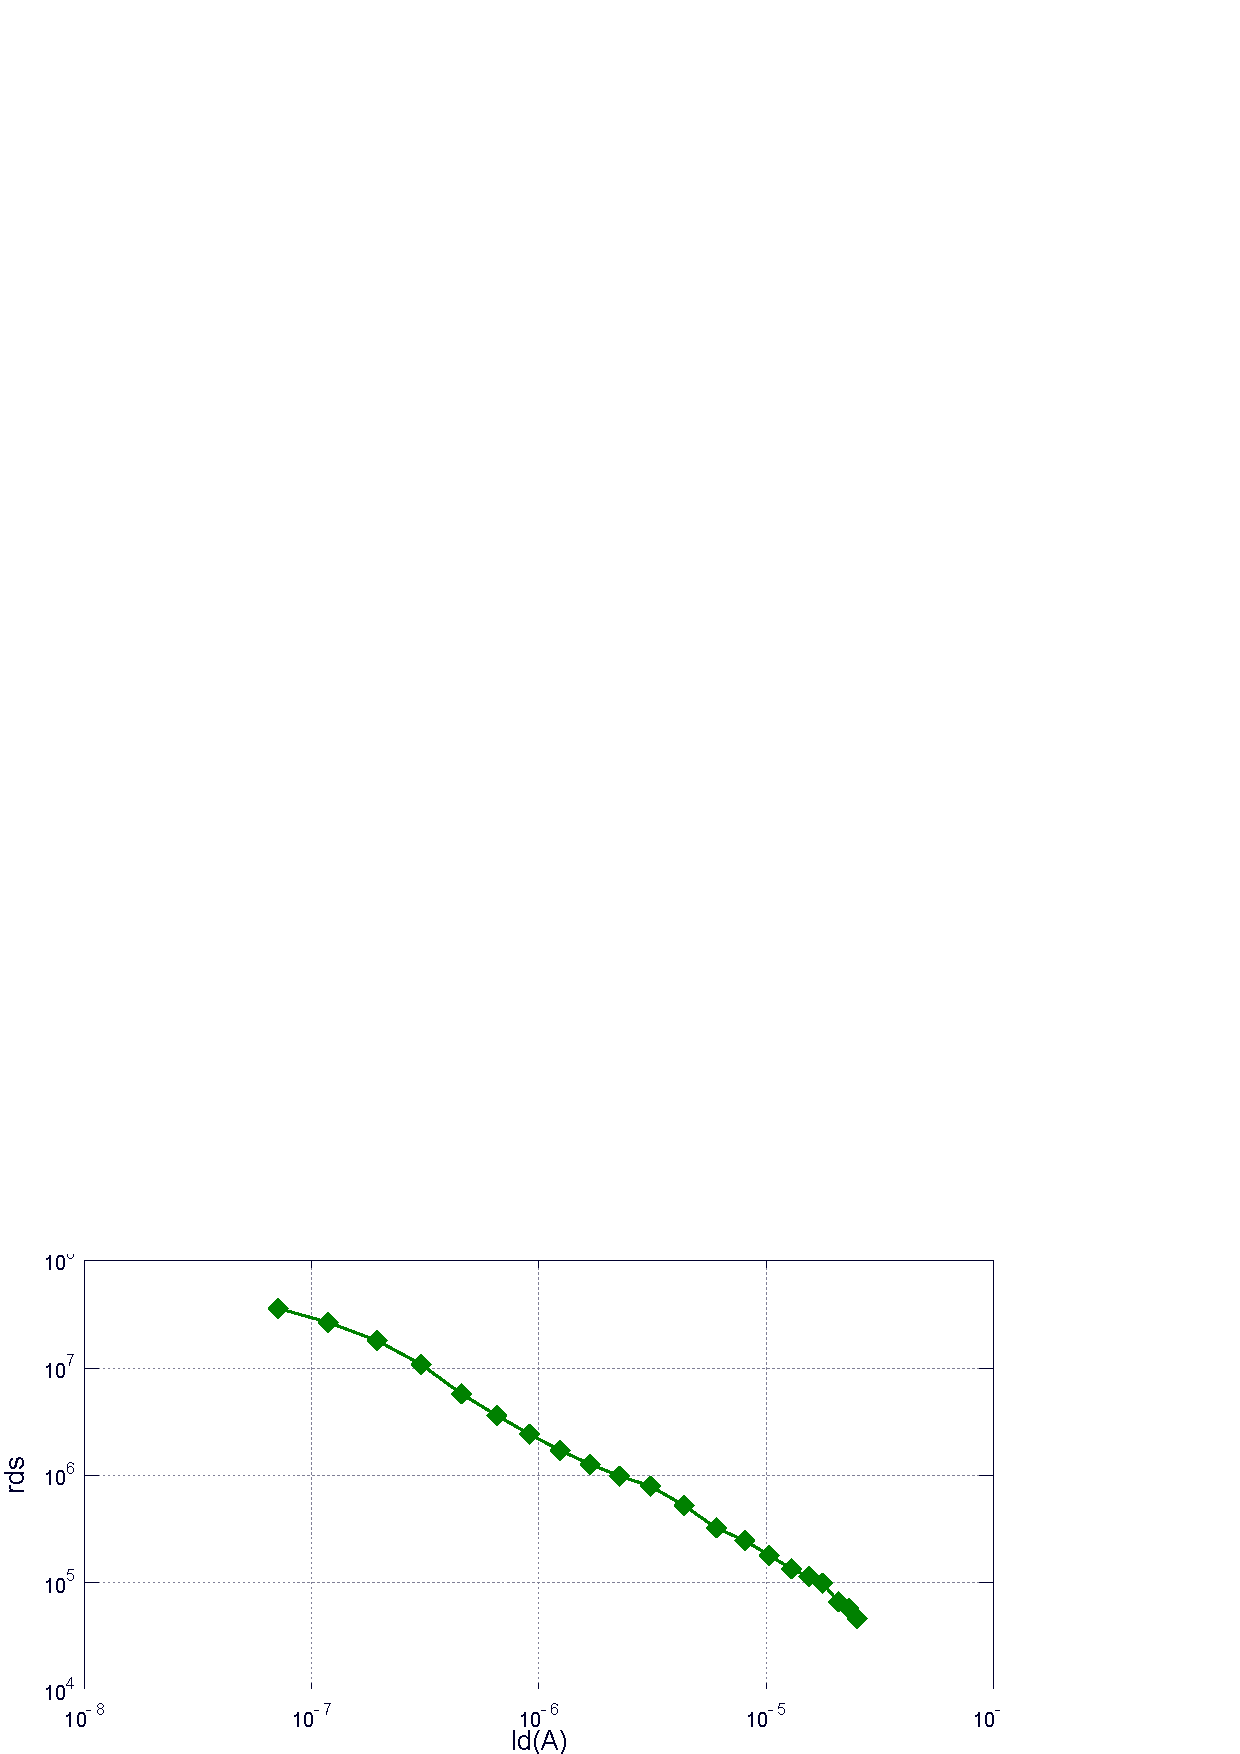
\includegraphics[width=0.8\textwidth]{images/chapter3/rds_I.png}
    \caption{Id-transconductance with Vds variance}
    \label{fig:rds}
\end{figure}


\section{Disparity}
We measured two nanowire elements which lie on the same wafer and are immersed with the same testing PBS solution.
Below the $g_m$-$I_D$ plot (Fig.\ref{fig:disparity}) shows that even the environment is same, two elements exhibit different electrical response.

\begin{figure}[!htbp]
    \centering
    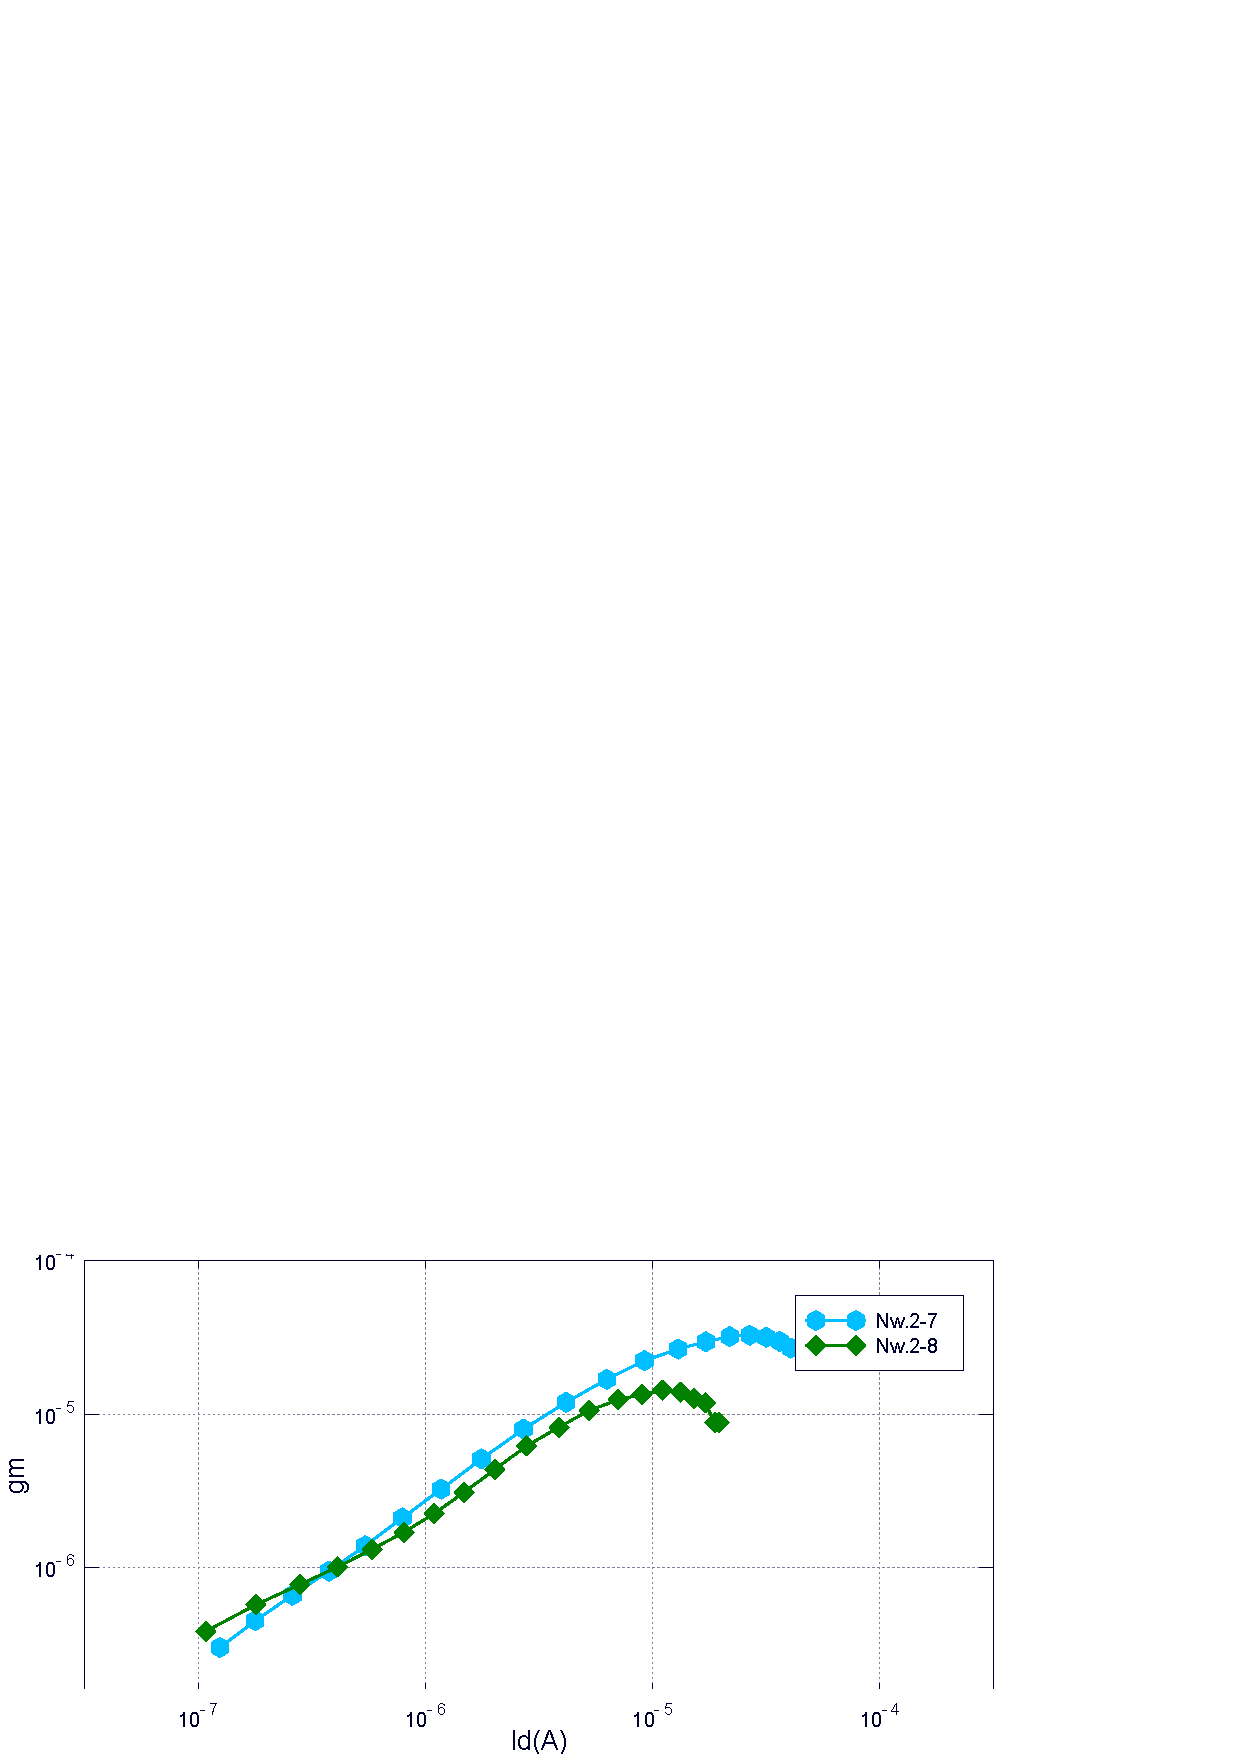
\includegraphics[width=0.8\textwidth] {images/pDisparity.png}
    \caption{Dusparity problem casue nanowire elements with same environment can exhibit different electrical responses.}
    \label{fig:disparity}
\end{figure}










 


\chapter{Discrete Circuitry Design}
This chapter contains the discrete circuit which has been briefly reviewed in section \ref{section:SF}.
We built this circuit to apply the constant current method to our nanowire element.

\section{Transforming the design from p-type measuring into n-type measuring}
In \cite{SF1}, the circuit is for p-type ISFET element (Fig.\ref{fig:SF_schematic_old}).
Our nanowire element is n-type.
Hence we transformed the circuit into the one in Fig.\ref{fig:SF_schematic}.
\begin{figure}[!htbp]
    \centering
    \includegraphics[width=0.8\textwidth] {../images/chapter4/SFdiscrete_old.png}
    \caption{The schematic of read-out circuit from \cite{SF1}. The ISFET is a p-type element. It is controlled by the current source $I_b$ whose sub-circuit is shown at right.}
    \label{fig:SF_schematic_old}
\end{figure}
\begin{figure}[!htbp]
    \centering
    \includegraphics[width=0.8\textwidth] {../images/chapter4/SFdiscrete_schematic.png}
    \caption{Our circuit schematic transformed from Fig.\ref{fig:SF_schematic_old}. The center transistor is a n-type element. It is controlled by the current source $I_b$ whose sub-circuit is shown at right.}
    \label{fig:SF_schematic}
\end{figure}


\section{Circuit Description}
The circuit is divided into two sections: the circuit body and the biasing current source (Ib).

\subsection*{Circuit Body}
The circuit body section is a source follower structure.
The input of the circuit is at the floating gate ($G$) of the center transistor, where the output is at its source-end ($S$).

The $I_D$ of the transistor is controlled by the Ib.
Because The leakage current flowing into the negative input of OP2 is less than 0.1nA, the $I_D$ of the transistor should always be same as the current provided by Ib.

The $V_{DS}$ is always equal to the potential difference ($I_0 \times R_0$) across the resistor $R_0$.
This is achieved by two OP-based unity gain buffer.
They connected serially with $R_b$ and cause the voltage at the drain-end ($D$) follows the voltage at the source-end ($S$).


\subsection*{biasing current source (Ib)}
The Ib is in fact a current scale down circuit.
By concerning the OP as ideal, the node $OP+$ has the same voltage with $OP-$.
This equalize the potential difference across two resistors whose resistance are different by $N$-fold.
As the result, the current of Ib and Is are also different by $N$-fold.
$I_b = I_s / N$.

The capacitor is for filtering. It filter the high frequency noise out to create a stable output current.


\section{Discrete Element}
We use tlc2264 made by Texas Instrument (TI) as our OP.
This OP element has working voltage of $\pm 5v$ and can perform rail-to-rail output operation.
Its gain (Large-signal differential voltage amplification rate) is 170 for the output load greater than 50k.

For the current source Is and I0, we use lm334 made by National Semiconductor.
It is a 3-terminal adjustable current sources with wide dynamic voltage range of 1v to 40v, and current accuracy of $\pm 3\%$.
In our experiment, the current $I_s$ is fixed at $1\mu A$ where its output impedance is $1.2G\Omega$.

\section{Circuit Performance and Conclusion}
We examined the performance of our circuit by plotting its $I_D$-$V_G$ curve.
The $I_0$, $R_0$ and $V_G$ were kept constant.
We swept the $I_D$ by changing the $N$ value with a variable resistor.
The $N$ ranges from 1 to 1000.
And the Ib circuit should produce bias current $I_b$ from $1\mu A$ to $1n A$.

We measured the output voltage at $S$ and subtracted this value from $V_G$ to get the respective $V_{GS}$.
These two value gave result to the $I_D$-$V_G$ curve in Fig.\ref{fig:SF_result}.
We compare this curve with the curve obtained by directly sweeping $V_G$ and measuring $I_D$ with Source Meter (Keithley 2602).

\begin{figure}[!htbp]
   \centering
   \includegraphics[width=0.8\textwidth]{images/chapter4/SF.png}
   \caption{The measuremet result (``SF\_measurement'') compares with the direct $I_D$-$V_G$ sweep (``Id-Vg sweep'').}
   \label{fig:SF_result}
\end{figure}

The result shows that when $I_D$ is larger than $10n A$, the circuit is functional.
Two curves are same as each other.

The circuit fails when $I_D$ is smaller than $10n A$.
This is caused by the unmatched impedance, which we have discussed in section.\ref{section:SF}.

The output impedance of Ib circuit is:
\begin{equation} \label{eq:rcs2_again}
    N\times R_s
\end{equation}
$R_s$ is the output impedance of current source Is which equals to $1.2G\Omega$.
And the current input impedance at the $S$ of the circuit body is:
\begin{equation} \label{eq:rsf2_again}
    \frac{1}{g_m}
\end{equation}

We plot the $I_D$-Impedance plot in Fig.\ref{fig:SF_imp}.

\begin{figure}[!htbp]
   \centering
   \includegraphics[width=0.8\textwidth]{../images/chapter4/SF_impedance.png}
   \caption{Input impedance of transistor (``1/gm'') and output impedance of Ib circuit (``Rs''). The former is found by the derivative of $I_D$ of $V_{Gs}$. The latter is obtained by Eq.\ref{eq:rcs2_again}.}
   \label{fig:SF_imp}
\end{figure}

It shows that the output impedance of Ib is close to the input impedance of transistor when current is $10n A$ (N = 100).
The impedance is unmatched.

Overall, the constant current method is feasible.
What one needs to notice when applying the constant current method is the impedance matching.
In source follower structure, its current input impedance varies with the bias current.
It effects the dynamic range and need more design concern.



\chapter{Integrated Circuitry Design}

\section{Signal Acquisition Method}


\chapter{Circuit Results Discussion and Summary}
This chapter presents the results of our read-out circuit and the summary of this thesis.

\section{The Fronted Circuit and DC-sweep mode}
\begin{figure}[tbh!]
    \centering
        \includegraphics[width=0.5\textwidth] {images/chapter6/FrontedCircuit.png}
    \caption{The fronted circuit}
    \label{fig:frontedCIrcuit}
\end{figure}
As in Fig.\ref{fig:frontedCIrcuit}(a), the fronted circuit includes a biasing current source (Ibias), transimpedance amplifier (TIA) and an operational amplifier (OP).
These three circuit blocks combined with the nanowire device (SiNW) form a feedback structure, which is DC-sweep mode of our circuit.

\subsection{The Output Current Range of Ibias Circuit}

\begin{figure}[tbh!]
    \centering
    \begin{minipage}[t]{0.25\textwidth}
        \includegraphics[width=1\textwidth] {images/chapter5/mirror.PNG}
        \raggedleft
    \end{minipage}
    \hfill
    \centering
    \begin{minipage}[t]{0.5\textwidth}
        \includegraphics[width=1\textwidth]{images/chapter6/Ibias.png}
        \raggedleft
    \end{minipage}
    \caption{\textbf{(a)} The Ibias circuit. \textbf{(b)} The relation between biasing current ($I_{bias}$) and resistance of the external resistor.}
    \label{fig:chip:mirror}
\end{figure}

The Fig.\ref{fig:chip:mirror}(a) is the schematic of the Ibias circuit.
The relation between the resistance of the external resistor and the biasing current is shown in Fig.\ref{fig:chip:mirror}(b).
The Ibias circuit is able to provide a biasing current from $100n A$ to $50\mu A$ stably.
It should be noted that this biasing current range binds the operational range of DC-sweep mode circuit.


\subsection{The Chip Measurement Results of TIA}
The Fig.\ref{fig:chip:TIA}(a) and (c) show that the dynamic input current range of TIA is $+5.3\mu A \sim -15\mu A$.
The Fig.\ref{fig:chip:TIA}(b) and (d) are the respective derivative ($\frac{\partial V_{out}}{\partial I_{in}}$)
As illustrated in these figures, the transimpedance of TIA is $103k$.
It is notable that not all TIA on the chips have the same transimpedance.
This is because the transimpedance value depends on the resistance of the resistor in TIA (Fig.\ref{fig:frontedCIrcuit}).
This resistor is made of N-well, which should have the largest resistance-to-surface ratio among other kinds of resistor.
But since the doping concentration may vary with the fabrication process, such kind of resistor has a larger resistance variance (\% 30).
We have performed necessary simulations before tap out.
It is assured that the variance does not disturb the important properties of whole read-out circuit such as stability and noise ratio.

\begin{figure}[tbh!]
    \centering
    \begin{minipage}[t]{0.65\textwidth}
        \includegraphics[width=1\textwidth]{images/chapter6/Trimp_I+.png}
        \raggedleft
    \end{minipage}
    \hfill
    \centering
    \begin{minipage}[t]{0.65\textwidth}
        \includegraphics[width=1\textwidth]{images/chapter6/Trimp_I-.png}
        \raggedleft
    \end{minipage}
    \caption{The dc simulation results of TIA. The x-axis represents positive/negative input current (log scale). \textbf{(a)} is the $V_{out}$ responding to the positive input current while \textbf{(c)} is to the negative input current.
                    \textbf{(b)} and \textbf{(d)} are the partial derivative of $V_{out}$ with respect to input current ($\frac{\partial V_{out}}{\partial {I_{in}}}$) from (a) and (c) respectively.}
    \label{fig:chip:TIA}
\end{figure}

\subsection{The Chip Measurement Results of the Feedback OP} \label{sec:ch6:OP}

A sinusoidal signal is sent to the negative input of OP and the output signal is measured in Fig.\ref{fig:chip:OPGain}.
It shows that the gain of the feedback OP is only about $1k$.
However, the gain of OP was designed to be more than $5k$.
We will discuss this problem in the following section.

\begin{figure}[tbh!p]
    \centering
        \includegraphics[width=0.7\textwidth] {images/chapter6/Problem_OPGain.png}
    \caption{The output voltage of the feedback OP when the negative input is applied with a sinusoidal signal.
            This input sinusoidal signal has frequency of $1$Hz and amplitude of $2m V$.
            The positive input of OP is biased with a constant voltage generated by the chip (VRef in Fig.\ref{fig:chip:DCmode}).
            The output signal has amplitude around $2 V$, which means that the gain of OP is about $1k$.}
    \label{fig:chip:OPGain}
\end{figure}

\subsection{Measurement with DC-sweep Mode Circuit and the Low-current Defect Problem}
\begin{figure}[h!tb]
    \centering
        \includegraphics[width=0.3\textwidth] {images/chapter6/DCMode.png}
    \caption{DC-sweep mode circuit}
    \label{fig:chip:DCmode}
\end{figure}

With DC-sweep mode (Fig.\ref{fig:chip:DCmode}), Ibias is swept and $V_G$ and $I_D$ are measured to obtain the $I_D$-$V_G$ and $I_{bias}$-$V_G$ curves (Fig.\ref{fig:chip:IdIbiasVG}).
The chip works well when $I_{bias}$ is larger than $1\mu A$.
The overlap between two curves implies that $I_D$ follows $I_{bias}$ and $V_G$ consequently alters owing to the feedback mechanism.
\begin{figure}[bt!]
    \centering
    \includegraphics[width=0.7\textwidth] {images/chapter6/gvt_0101Manual_IdVg.png}
    \caption{The measurement result of DC-sweep mode circuit. $I_{bias}$ is the biasing current. $I_D$ is the current flowing through the nanowire device.
    One can observe a separation between two curves in low current section ($< 1\mu A$).}
    \label{fig:chip:IdIbiasVG}
\end{figure}

When current becomes low, the circuit fails to prompt nanowire to follow the biasing current.
This phenomenon could be reasonable because lower $I_D$ implies lower $g_m$ and the feedback ability of the circuit may be not strong enough to push the gate of nanowire.
However, we expected this happens for $g_m$ below $200n$.
The Fig.\ref{fig:chip:gmId} indicates that the this happens when $g_m$ is less than $5\mu$ instead.
We call this problem as low-current defect problem.
\begin{figure}[tbh!]
    \centering
    \includegraphics[width=0.6\textwidth] {images/chapter6/gvt_0101Manual_gmId.png}
    \caption{The $g_m$-$I_D$ curve. It is obtained from the $I_D$-$V_G$ curve in Fig.\ref{fig:chip:IdIbiasVG}.
    ``Circuit fails'' means the two curves in Fig.\ref{fig:chip:IdIbiasVG} are separated where ``circuit works'' means they are overlapped.}
    \label{fig:chip:gmId}
\end{figure}

\subsubsection*{Insufficient Gain}
We first suspected that it is caused by the insufficient gain of the feedback OP.
According to the last section (Section.\ref{sec:ch6:OP}), the gain is about $1k$.
The discussion in Section.\ref{sec:feedM} suggests that the feedback mechanism depends on the loop gain.
The loop gain should be larger than 100 for DC-sweep mode being functional.
Based on Eq.(\ref{eq:TF_RA}) and Eq.(\ref{eq:TF_LG}), if $A_{OP}$ is $1k$, the loop gain drops below 100 when $g_m$ is less than $1\mu$.
In other words, even though the gain of OP is 5 fold smaller than the gain we designed, the circuit should work well when $g_m$ is larger than $1\mu$.
But in fact, the circuit fails for $gm$ below $5\mu$.



\begin{figure}[tbh!]
\centering
    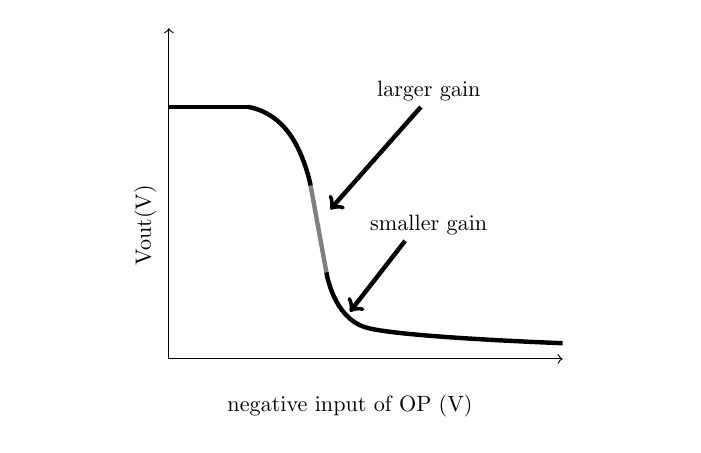
\begin{tikzpicture}
        \draw [black, ultra thick] plot coordinates { (0,4) (1,4) };
        \draw [black, ultra thick] plot [smooth, tension=1] coordinates { (1,4) (1.5,3.7) (1.8,3) };
        \draw [gray, ultra thick] plot [smooth, tension=1] coordinates { (1.8,3) (2,1.9) };
        \draw [black, ultra thick] plot [smooth, tension=0.5] coordinates { (2,1.9) (2.5,1.2) (5, 1) };

        \draw[->] (0, 0.8) -- (0, 5);
        \draw[->] (0, 0.8) -- (5, 0.8);
        \draw[->, ultra thick] (3.2, 4) -- (2.05,2.7);
        \draw[->, ultra thick] (3, 2.3) -- (2.3,1.4);
        \node[text width=5cm, scale=0.8, align=center] at (3.3, 2.5)
            {smaller gain};
        \node[text width=5cm, scale=0.8, align=center] at (3.3, 4.2)
            {larger gain};
        \node[text width=10cm, scale=0.8, align=center] at (2.3, 0.2)
            {negative input of OP (V)};
        \node[text width=5cm, scale=0.8, align=center, rotate=90] at (-0.3, 2.5)
            {Vout(V)};
    \end{tikzpicture}
    \caption{The illustration of the input-output response of the feedback OP.}
    \label{fig:chip:line}
\end{figure}


\subsubsection*{Input Offset Voltage}
Another reason may be responsible for the low-current defect is the offset voltage at the input of the feedback OP.

The output voltage of TIA ($V_{TIA}$) of the DC-sweep experiment in Fig.\ref{fig:chip:IdIbiasVG} is examined and shown in Fig.\ref{fig:chip:VTIA}.
Ideally, when feedback mechanism works well, $V_{TIA}$ should be equal to $V_{Ref}$(Fig.\ref{fig:chip:DCmode}).
However, the value of $V_{Ref}$ is $0.802 V$, which is smaller than $V_{TIA}$.
(This $V_{Ref}$ is connected to a constant voltage point inside the chip.
its value is known indirectly by measuring the drain voltage of nanowire since the drain of nanowire is kept to be same as $V_{Ref}$ by TIA.)
When the circuit works well, $V_{TIA}$ and $V_{Ref}$ is still different by $15m V$.
This voltage difference can result in a $150n A$ offset current flowing through TIA and into the nanowire device.
This offset current becomes remarkable when the $I_{bias}$ becomes small.

We suggest the reason that $V_{TIA}$ is large than $V_{Ref}$ is due to the offset voltage appearing at the input of the feedback OP.
This speculation is reasonable with respect to the layout, which will be discussed in the next section.

\begin{figure}[tbh!]
    \centering
        \includegraphics[width=0.7\textwidth] {images/chapter6/gvt_0101Manual_VopiProblem.png}
    \caption{The $V_{TIA}$. The x-axis is the corresponding gate voltage.
                With the information from Fig.\ref{fig:chip:IdIbiasVG}, we found that the $V_{TIA}$ is not equal to $V_{Ref}$ no matter feedback mechanism works well or not.}
    \label{fig:chip:VTIA}
\end{figure}

Overall, the insufficient gain and the input offset may be the main reasons of the low-current defect.
Both of them relate to the feedback OP.
We then discuss these two reasons from the perspective of layout in the following section.

\subsection{The Layout Problems of OP}
The last section mentioned that the gain of OP is lower than we expected and there may exist an input offset voltage.
In this section, we will deduce that several layout flaws may be responsible for these two problems.

\begin{figure}[tbh!]
    \centering
    \includegraphics[width=1\textwidth] {images/chapter6/OP_schematic.png}
    \caption{The left section is the schematic of the feedback OP including the local biasing circuit and OP circuit. The right section is the global biasing circuit for generating two global biasing voltages: $V_{bi}$, $V_{Ref}$.
                The Iin is an external current source.}
    \label{fig:chip:OPScem}
\end{figure}

\begin{figure}[tbh!]
    \centering
    \includegraphics[width=0.7\textwidth] {images/chapter6/TrOP_layout.PNG}
    \caption{The layout of the feedback OP including the local biasing circuit. }
    \label{fig:chip:OPLayout}
\end{figure}

\subsubsection{The Possible Reasons for Insufficient Gain}
The schematic presented in Fig.\ref{fig:chip:OPScem} contains two sections.
The left section is the body of the feedback OP and the local biasing circuit while the right one is a global biasing circuit.
The global biasing circuit generated $V_{bi}$ and $V_{Ref}$, which bias two pmos (M3, M4) and two nmos (M5, M6) respectively.

One layout flaw is that the M3 $\sim$ M6 are all single transistor.
They are placed alone on the chip (Fig.\ref{fig:chip:OPLayout}) without any protection.
In consequence their size and doping concentration are more vulnerable to the process variation than other transistors.
Another layout flaw is that the global biasing circuit is placed far from the OP circuit.
The extent of the process variation from which the OP circuit and global biasing circuit suffer may be different.

Take an example, when process variation happens in global biasing circuit, $V_{bi}$ and $V_{Ref}$ change respectively.
Ideally, the effect of these two changes on the gain of OP are countervailing.
But this may not be true if M4 and M6 suffer another process variation.
The changes on $V_{bi}$ and $V_{Ref}$ may affect M4 and M6 in different extent.
Moreover, the high output impedance of OP amplifies this difference and as a result of the gain distortion.

\subsubsection{The Possible Reasons for Input Offset}
The input offset can be related to the size mismatch between M7 and M8 (Fig.\ref{fig:chip:OPLayout}).
The transistors were designed to be same.
But there is no dummy gate or matching technique applied to the transistors.
Therefore, the size mismatch may prone to happen on M7 and M8.
In our case, the offset voltage is negative ($V_{\text{negative input}} > V_{\text{positive input}}$).
If the size mismatch is responsible for it, the size of M8 should be relatively smaller than M7.

\subsubsection{Improvement Methodology}
Although all problems mentioned above relate to the layout, we do not think that simply revising the layout is a reliable solution.
The feedback OP is an open-loop circuit with high output impedance.
Its characteristics (such as gain and bandwidth) are hard to be control accurately considering the process variations.
A better solution is to replace it with other amplifier.
Since this OP serves as a high-gain and low bandwidth block, it can be substitued with a close-loop amplifier and low pass filter.

\subsubsection{Summary of DC-sweep mode}
The table that compares the chip properties and the specification for DC-sweep mode is given below (Table.\ref{tb:chip:gvtR}).
The chip does not meet the specification due to the low-current defect problem.


\begin{table}[tbh!]
    {\fontfamily{}\fontsize{10}{14}\selectfont
    \centering
    \begin{tabular}{l|c|c}
        & Design Spec. & Chip Properties  \\
        $I_D$ & $100n A$ - $30\mu A$ & $1\mu A$ - $50\mu A$ \\
        \hline
        $g_m$ & $200n A$ - $20\mu A$& $3\mu $ - $20\mu A$\\
        \hline
        $V_G$ & $0.5V$ - $3V$ &  $0.45V$ - $3V$\\
    \end{tabular}
        \caption{The comparison between the chip properties and the specification for DC-sweep mode from chapter 3.}
        \label{tb:chip:gvtR}
    }
\end{table}

\section{The Second Stage Circuit and Transient Measurement Mode}
\begin{figure}[tb!hp]
    \begin{minipage}[t]{0.5\textwidth}
        \centering
        \includegraphics[width=1\textwidth]{images/chapter6/NWROC_block.png}
        \raggedleft
        (a)
    \end{minipage}
    \hfill
    \begin{minipage}[t]{0.5\textwidth}
        \centering
        \includegraphics[width=1\textwidth]{images/chapter6/Second.png}
        \raggedleft
        (b)
    \end{minipage}
    \caption{\textbf{(a)} The block diagram of Transient Measurement circuit. \textbf{(b)} The schematic of the second stage circuit.}
    \label{fig:chip:ACschem}
\end{figure}

As in Fig.\ref{fig:chip:ACschem}, Transient Measurement mode includes the second stage circuit and the Ibias and TIA from the fronted circuit.
An analog subtractor and a resistor-based amplifier are included in the second stage circuit.
The input signal can be sent from the gate or the source of nanowire (SiNW).




\subsection{The Second Stage Circuit}
This section presents the important properties of the second stage circuit.
To be notable that the performance of the subtractor and amplifier cannot be measured independently because there is no external pad connected to the output of the subtractor.
Besides, second stage input is always connected with the output of TIA.
Due to the low output impedance of the TIA, it is hard to send input signal into the second stage circuit directly.
Fig.\ref{fig:chip:MeasMethod} is the alternative approach.
The resistor Rs and the TIA compose a voltage amplifier.
The input signal, which is usually triangular or sinusoidal, is injected through the Rs.
It is then modulated in proportional to the ratio of Rs and TIA before being sent into the second stage circuit.
\begin{equation}
    {\text{Input of the }2^{nd}\text{ stage circuit} = V_s \times \frac{\text{transimpedance of TIA}}{R_s}}
\end{equation}

\begin{figure}[tbh!]
    \centering
    \includegraphics[width=0.7\textwidth] {images/chapter6/CVMVsMeas.png}
    \caption{The second stage circuit measurement approach.}
    \label{fig:chip:MeasMethod}
\end{figure}



\subsubsection{The Noise Oscillation Problem in Amplifier with Amplification Rate of 1  }
The amplifier in the second stage circuit has three amplification rate ($A_{amp}$): 1, 10 and 100.
The amplifier works well as the $A_{amp}$ is 10 and 100.
However, when $A_{amp}$ is 1, the output signal is flooded with noise.
In Fig.\ref{fig:chip:ss_noise}, the input is a 1Hz triangle signal.
Ideally, the second stage output should be a similar triangle signal.
But in fact the signal is flooded with noise.
\begin{figure}[tbh!]
    \centering
    \includegraphics[width=1\textwidth] {images/chapter6/Subtractor_noise.png}
    \caption{The noise ocsillation problem}
    \label{fig:chip:ss_noise}
\end{figure}

We suggest that the oscillation of noise signal should be the main cause of the problem.
When designing the amplifier, we did not consider the parasitic capacitance brought by the switches and the pad (with ESD circuit) at the output.
The simulation below proves our suggestion.
The parasitic capacitance is modeled by a $5p F$ capacitor.
Fig.\ref{fig:chip:pMsim}(a) and (b) are the phase margin test of the amplifier before and after the capacitor is loaded on the output.
The figures indicate that the second dominant pole locates at the output and the parasitic capacitors push it to the left.
The phase margin is decreased subsequently.


\begin{figure}[tb!h]
    \centering
    \makebox[0.8\linewidth][r]{(a)}
    \begin{minipage}[t]{1\linewidth}
        \centering
        \includegraphics[width=0.7\linewidth] {images/chapter6/Amp_PM.PNG}
    \end{minipage}
    \centering
    \makebox[0.8\linewidth][r]{(b)}
    \begin{minipage}[t]{1\linewidth}
        \centering
        \includegraphics[width=0.7\linewidth] {images/chapter6/Amp_PM_5p.PNG}
    \end{minipage}
    \caption{The post-simulation of the phase margin test of the amplifier when amplification rate is 1.
            \textbf{(a)} Without the parasitic capacitor, the phase margin is 108 degree.
            \textbf{(b)} With the parasitic capacitor (modeled by a $5p F$ capacitor), the phase margin becomes 30 degree.}
    \label{fig:chip:pMsim}
\end{figure}



\begin{figure}[tbh!]
    \centering
    \includegraphics[width=1\textwidth] {images/chapter6/SeconStage_feed.png}
    \caption{The feedback network and loop gain computation structure of the amplifier with \textbf{(a), (b)} $A_{amp} = 1$ and \textbf{(c), (d)} $A_{amp} = 10$ or $100$.}
    \label{fig:chip:ss_feed}
\end{figure}

The reason that the noise oscillation problem only happens when $A_{amp}$ is 1 is because of the feedback mechanism.
When $A_{amp}$ is 1, the structure is similar to an unit-gain buffer (Fig.\ref{fig:chip:ACschem}(b)).
In Fig.\ref{fig:chip:ss_feed}, (a) is the feedback network of this structure while (c) is of the amplifier with $A_{amp}$ is 10 and 100.
To compute the loop gain, the structure is broken at the negative input and a tested signal is injected ($Vt$) as illustrated in Fig.\ref{fig:chip:ss_feed} (b), (d).
The loop gain ($\frac{V_f}{Vt}$) of the two structure is derived as:
\begin{align}
    & \text{when $A_{amp} = 1$:} && \frac{V_f}{Vt} = A_{op} \\
    & \text{when $A_{amp} = 10$ or $100$:} && \frac{V_f}{Vt} = A_{op} \times \frac{R_i}{R_i + R_o}
\end{align}
$A_{op}$ is the gain of the OP in the amplifier.
($A_{op}$ is similar in two cases even if the loading effect is taken into consideration becasue $R_O >> R_i$.)
Since the $R_O$ is at least larger than $R_i$ by 10-fold, two loop gains are different by 10-fold as well.
The smaller loop gain increases the phase margin of amplifier by about 45 degree and diminish the oscillation (Fig.\ref{fig:chip:pMsim_10x}).

\begin{figure}[tbh!]
    \centering
    \includegraphics[width=0.7\textwidth] {../images/chapter6/Amp_pm_5p_10x.PNG}
    \caption{The post-simulation of the phase margin test of the amplifier when amplification rate is 10.
                With the parasitic capacitor loaded on the output(modeled by a $5p F$ capacitor), the phase margin is 73 degree}
    \label{fig:chip:pMsim_10x}
\end{figure}

We tried to dealt with the noise oscillation problem by the signal average technique.
The output signal is averaged out to remove the noise component.
However, the average of the signal may lie on the wrong offset.
Therefore, the amplifier with $A_{amp} = 1$ is used only when the signal trend is of interest (such as the dynamic input range in Section.\ref{sec:DIR}).
When the output signal is large and the amplification is not necessary, we simply measure the output of TIA.





\subsubsection{Dynamic Input Range} \label{sec:DIR}
Fig.\ref{fig:chip:xin} is the input-output response of the second stage circuit ($A_{amp} = 1$).
It is used for finding the dynamic input range of the circuit.
The linear region locates at $Vin = 0.43V \sim 1.32V$.
According to chapter 5, this range is determined by the subtractor block.
\begin{figure}[tbh!]
    \centering
    \includegraphics[width=0.6\linewidth] {images/chapter6/SubtractorXin.png}
    \caption{The input-output response of the second stage circuit ($A_{amp} = 1$).}
    \label{fig:chip:xin}
\end{figure}

Another input of the circuit is the Vz (Fig.\ref{fig:chip:ACschem}(b)).
This voltage is for shifting the offset voltage.
Its dynamic input range is measured and presented in Fig.\ref{fig:chip:zin}, which ranges from $0.62V$ to $1.47V$.
To be notable that ideally the input Vz should be equal to the output.
But in fact an offset voltage of $0.15V$ occurs in Fig.\ref{fig:chip:ACschem} due to the noise oscillation problem mentioned in the last section.
This offset does not exist when the $A_{amp}$ is 10 and 100.
\begin{figure}[tbh!p]
    \centering
    \includegraphics[width=0.6\linewidth] {images/chapter6/SubtractorZoffset.png}
    \caption{The input-output response of the second stage circuit. The input is Vz, which decides the output offset of the circuit.}
    \label{fig:chip:zin}
\end{figure}

\subsubsection{The Circuit Gain}
A triangle wave is sent to the end of Rs (Fig.\ref{fig:chip:MeasMethod}) and the input and output of the second stage circuit are recorded by an oscillation scope.
Fig.\ref{fig:chip:amp}) (a), (b) and (c) are the time domain results when the $A_{amp}$ is 1, 10 and 100 respectively.
The exact gain values are summarized in the Table.\ref{tb:chip:ampGain}.


\begin{figure}[tbh!p]
    \centering
    \begin{minipage}[t]{1\linewidth}
        \centering
        \includegraphics[width=0.8\linewidth] {images/chapter6/SubtractorXin_scope.png}
        (a)
    \end{minipage}
    \centering
    \begin{minipage}[t]{1\linewidth}
        \centering
        \includegraphics[width=0.8\linewidth] {images/chapter6/SecondStageAmp10x.png}
        (b)
    \end{minipage}
    \begin{minipage}[t]{1\linewidth}
        \centering
        \includegraphics[width=0.8\linewidth] {images/chapter6/SecondStageAmp100x.png}
        (c)
    \end{minipage}
    \caption{The input output signal of the second stage circuit in time domain when $A_{amp}$ is \textbf{(a)} 1, \textbf{(b)} 10 and \textbf{(c)} 100.}
    \label{fig:chip:amp}
\end{figure}

\begin{table}
    {\fontfamily{}\fontsize{10}{14}\selectfont
    \centering
    \begin{tabular}{l|c|c|c}
        Designed Amplification Rate & 100 & 10 & 1 \\
        \hline
        Measured Amplification Rate & 93.3 & 9.2 & 1 \\
        \hline
        Error Rate & 7.7 \% & 8 \% & 0 \\
    \end{tabular}
    \caption{Comparison between the desgined and measured gain of the second srage circuit.}
    \label{tb:chip:ampGain}
    }
\end{table}

\subsection{Transient Measurement Mode}
The second stage circuit and the TIA from the fronted circuit compose the circuit of Transient Measurement Mode.
This section presents some of its important properties (gain, noise and bandwidth).



\subsubsection{Bandwidth and Gain}

\begin{figure}[tbh!p]
    \centering
    \begin{minipage}[t]{1\linewidth}
        \centering
        \includegraphics[width=0.8\linewidth] {images/chapter6/Bw_10x.png}
        (a)
    \end{minipage}
    \centering
    \begin{minipage}[t]{1\linewidth}
        \centering
        \includegraphics[width=0.8\linewidth] {images/chapter6/Bw_100x.png}
        (b)
    \end{minipage}
    \caption{The gain and bandwidth of Transient Measurement circuit. The $A_{amp}$ is 10 in \textbf{(a)} and 100 in \textbf{(b)}.}
    \label{fig:chip:bw}
\end{figure}
The gain is the input current to output voltage ratio.
Because the noise oscillation problem may disturb the bandwidth measurement, we did not measure the circuit with $A_{amp}$ of 1.
The circuit with $A_{amp}$ of 10 has gain of $891k$ and -3dB bandwidth of $30k$Hz.
The circuit with $A_{amp}$ of 100 has gain of $8.9M$ and -3dB bandwidth of $7.5k$Hz.

\subsubsection{Input Referred Noise}
The spectrum analyzer are used to measure the noise.
The power spectral density (PSD) of noise at the output of the circuit is measured and is referred to the input to show the equivalent input current noise (Fig.\ref{fig:chip:noise}).
Due to the equipment setting, the noise measring between $10$Hz and
While measurement is performing, Ibias provides $10\mu A$, which is same to the condition of the post-simulation measurement (Fig.\ref{fig:sim:vgnoise}).
The primary type of noise are the low frequency noise (flicker noise).
Other types of noise such as $60$Hz come from the environment and working machines.
They may be lowered by adopting better method of experiment or equipments.
Overall, the amount of noise is tolerable.
The input current noise is $0.3n A$ at 1 Hz.
The spec. from chapter 3 allows for a maximal input current noise of $2n A$.

\begin{figure}[tbh!p]
    \centering
    \includegraphics[width=0.8\linewidth] {images/chapter6/Noise.png}
    \caption{Input referred noise of Transient Measurement circuit.}
    \label{fig:chip:noise}
\end{figure}

\subsubsection{The Detection Range}
The spec. of our design demand a detection range for input current of $\pm 20n A \sim \pm 2.8\mu A$.
The upper bound of the current detection is decided by the TIA circuit, which is $5.3\mu A$ and $15 \mu A$.
The lower bound mainly relates to the noise.
We find the lower bound by sending a pulse input to the gate of nanowire.
This input voltage induced a current variance ($\Delta I_D$) and resulted in a pulse signal at output.
We then used oscilloscope to see how low the $\Delta I_D$ can be when it is still possible to detect it through the output.

\begin{figure}[tbh!p]
    \centering
    \begin{minipage}[t]{1\linewidth}
        \centering
        \includegraphics[width=0.8\linewidth] {images/chapter6/VinToVout_scope_0425_150mV.png}
        (a)
    \end{minipage}
    \centering
    \begin{minipage}[t]{1\linewidth}
        \centering
        \includegraphics[width=0.8\linewidth] {images/chapter6/VinToVout_scope_0425_20mV.png}
        (b)
    \end{minipage}
    \caption{}
    \label{fig:chip:DR_scope}
\end{figure}

The Fig.\ref{fig:chip:DR_scope}(a) and (b) are the output signals when the amplitude of input pulse signals are $150m V$ and $20m V$ respectively.
The current variance induced in two cases are $28n A$ and $2.8n A$
The high and low value can be barely distinguished in \ref{fig:chip:DR_scope}(b).
Therefore, we say the lower bound of our circuit is $\pm 2.8n A$. (The positive input and negative)
This matches the noise measurement in the last section.
The noise is $0.3n A$ and the detecting range is ten-fold larger than that value.

\subsubsection{Modulating biomolecule signals from the source terminal} \label{sec:ch6:Modulating}
The second usage of Transient Measurement mode is to apply a sinusoidal signal at the source of nanowire.
In Fig.\ref{fig:chip:sin}, is obtained by this measurement method.
The input is a sinusoidal signal with frequency of $500$Hz and the amplitude of $0.5V$.
The nanowire was put under two solutions with different pH values in (a) and (b).
After dividing the amplitude of the output signal by the transimpedance gain of the circuit (891k), we learned that the $g_m$ of nanowire under these two pH solutions are $1\mu$ and $1.8\mu$.

This method aims to modulate the biomolecule signal into higher frequency to avoid the flicker noise and other kinds of low frequency noise.
However, from the result below, it can be observed that the output contains large amount of high frequency noise.
We believe the noise comes from the testing solution and through the gate of nanowire.
In the future, a bandpass filter with adjustable center frequency should be added to the circuit to filter the signal of the unwanted frequency.

\begin{figure}[tbh!p]
    \centering
    \begin{minipage}[t]{1\linewidth}
        \centering
        \includegraphics[width=0.8\linewidth] {images/chapter6/Sin_1u.png}
        (a)
    \end{minipage}
    \centering
    \begin{minipage}[t]{1\linewidth}
        \centering
        \includegraphics[width=0.8\linewidth] {images/chapter6/Sin_1p8u.png}
        (b)
    \end{minipage}
    \caption{The output signal of the measurement using source of nanowire as input.
            The $gm$ of nanowire in two figures are different by using testing solution with different pH values.
             The $gm$ of nanowire is $1\mu$ in \textbf{(a)} and $1.8\mu$ in \textbf{(b)}.  }
    \label{fig:chip:sin}
\end{figure}


\subsubsection{Summary of Transient Measurement mode}
The Table.\ref{tb:chip:cvmR} compares the chip properties and the specification for transient measurement mode.
Although there is the noise oscillation problem, the performance of the circuit is fine.

\begin{table}[tbh!]
    {\fontfamily{}\fontsize{10}{14}\selectfont
    \centering
    \begin{tabular}{l|c|c}
        & Design Spec. & Chip Properties  \\
        \hline
        \hline
        IBias Current ($I_D$)& $600n A$ - $5\mu A$ & $100n A$ - $50\mu A$\\
        \hline
        Dynamic Input Current Range($\Delta I_D$) & $\pm 20n A$ - $\pm 2.8\mu A$ &
        \begin{tabular}{@{}c@{}}
            $2.8n A \sim 5.3\mu A$ \\ $-15\mu A\sim -2.8n A$
        \end{tabular}\\
        \hline
        Input Referred Noise (A) &$< 2n A$ & $< 0.3n A$ @ $1$Hz\\
        \hline
        Transimpedance Gain (max) & $5 M(\frac{V}{A})$& $8.9 M (\frac{V}{A})$\\
        \hline
        Bandwidth &$> 1k$ (Hz) & $7.5k Hz$\\
    \end{tabular}
        \caption{The comparison between the chip properties and the specification for Transient Measurement mode from chapter 3.}
        \label{tb:chip:cvmR}
    }
\end{table}


\section{Dealing with the Device Variability Problem} \label{sec:ch6:dvp}
This section presents the measurement with the proposed variability-resisting method.

Two nanowire devices (nw1-2, nw2-1) lying on the same substrate are under test.
The $I_D$-$V_G$ curves of two devices are obtained and substantiate that they have device variability problem (Fig.\ref{fig:chip:DeviceVar}(a)).
These curves are then transformed into $gm$-$Id$ curves (Fig.\ref{fig:chip:DeviceVar}(b)).
Based on the conclusion of appropriate operation region (Section.\ref{section:biasVg}), the $gm$ of $2\mu$ is selected.
The certain $I_D$ under which devices are biased are therefore determined.
As illustrated in Fig.\ref{fig:chip:DeviceVar}(b), nw1-2 is biased under $340n A$ and nw2-1 is biased under $900n A$.
The devices are connected with the circuit in Transient Measurement mode, where the bias current and gate voltage are set.
Finally, the output response of two devices are presented in Fig.\ref{fig:chip:DeviceVar}(c) and (d).
Two solutions with different pH values is used in substitution for the DNA solution.
The pH value of solution A is lower than solution B.
The lower pH value means the solution is more positive.
Thus, solution B increase $I_D$ and increases output voltage.


\begin{figure}[bth!]
    \centering
    \begin{minipage}[t]{0.4\linewidth}
        \includegraphics[width=1\textwidth] {images/chapter6/DeviceVar_IdVg.png}
        \raggedleft (a)
    \end{minipage}
    \centering
    \begin{minipage}[t]{0.55\linewidth}
        \includegraphics[width=1\textwidth] {images/chapter6/DeviceVar_gmId.png}
        \raggedleft (b)
    \end{minipage}
    \begin{minipage}[b]{1\linewidth}
        \includegraphics[width=1\textwidth] {images/chapter6/DeviceVar_scope.png}
        \makebox[0.4\linewidth][r]{ (c)}
        \makebox[0.57\linewidth][r]{ (d)}
    \end{minipage}
    \caption{The variability-resisting method.}
    \label{fig:chip:DeviceVar}
\end{figure}

Two devices have similar output response, which suggest our method is functional.
But still the responses are not exactly same.
The voltage difference appears in the are different by 8\% ($\frac{(|\Delta V_1 - \Delta V_2|)}{\Delta V_1}$).
We can blame the inaccurate biasing current because DC-sweep mode circuit fails in low current and the $V_G$ is manually adjusted to make the $I_D$ follows the biasing current.
Still there may be other reasons.

Although we keep the devices under a same $gm$, the output signals can diverge if they receive incomparable input.
The input of the experiment above is the equivalent voltage change induced by the concentration (pH value) difference ($\Delta V$).
Its value may be different because of two reasons.
One is that the thickness of the each nanowire may not be same.
There may be corrosion of the nanowire surface since the devices we use have been produced for more than 2 years and have bedd used repeatedly.
The other is the gate coupling effect.
The effect caused by the double layer capacitance varies with the gate voltage, which we have mentioned in Section.\ref{sec:assumpDiscuss}.

The first reason can be solved by producing a new device.
The second reason need the improvement on circuit structure.
This reminds us one of the advantages of source follower structure (Section.\ref{section:SF}).
The structure keeps $V_G$ constant and adjusts the source voltage of nanowire instead.
But changing source voltage will as well change the drain-to-source voltage ($V_{DS}$) of nanowire, which brings about the short channel effect.
Therefore, in the future, if our circuit adopts the concept of source follower, the additional feedback network that keeps $V_{DS}$ constant is required.

Overall, although our method does not entirely remove the device variability problem, it mitigates the problem.
Furthermore, the improvement method is proposed and the progress can be looked forward.

\section{Conclusion and Future Work}
\begin{figure}[!htb]
    \centering
    \includegraphics[width=0.7\textwidth] {images/chapter6/layout.PNG}
    \caption{The layout of the Readout circuit}
    \label{fig:layout}
\end{figure}
Fig.\ref{fig:layout} is the chip layout of the circuit.
It contains four unit of the read-out circuits and is able to measure four nanowire devices at the same time.

In this project, a circuit with two mode: DC-sweep mode and Transient Measurement mode is designed.
The first mode is to perform $I_D$-$V_G$ sweep while the second mode is to perform transient measurement.
By combining two mode, the circuit perform measurement by the variability-resisting method we proposed in this project.
This method mitigate the device variability problem and can be further improve in the future.
In Table.\ref{tb:ConcCompare}, our circuit is compared with the methods that were reviewed in chapter 2 \cite{Juv2}, \cite{Jlockin}.
Our circuit has wider $\Delta I$ detection range and lower power consumption when comparing with the similar work \cite{Jlockin}.
The work in \cite{Juv2} has better performance over all.
Still our circuit deals with the device variability problem, which does not be mentioned in both works.

\begin{table}[!htb]
    {\fontfamily{}\fontsize{10}{14}\selectfont
    \centering
    \begin{tabular}{l|c|c|c}
        & \cite{Juv2} & \cite{Jlockin} & This work \\
        \hline
        $\Delta I$ &  $120\mu A \sim 0.12n A$ & $3\mu A \sim 60n A$ &
                \begin{tabular}{@{}c@{}}
                    $3n A \sim 5.3\mu A$ \\ $-15\mu A\sim -3n A$
                \end{tabular}
                \\
        \hline
        Power consumption & 14.82uW & 2mW & 1.48mW\\
        \hline
        CMOS Technology & 0.13um & 0.18um & 0.35um\\
        \hline
        Device Variability & No Discussion & No Discussion & Variability-resisting method \\
    \end{tabular}
    \caption{Specification Summary}
    \label{tb:ConcCompare}
    }
\end{table}




\subsection{Future Work}
\paragraph{Problems in the Circuit Design}
The low current defect in DC-sweep mode is the most important problem that must be solved.
The solution for it is to replace the feedback OP with other closed-loop amplifier.
Another problem is the noise oscillation problem that happens when the $A_{amp}$ of the amplifier in the second-stage circuit is 1.
This problem can be solved simply by fixing the insufficient phase margin.

\paragraph{Introduce Filter and Better Experimental Process}
The noise included in Transient Measurement mode could be removed by simply introduce a bandpass filter.
The problem of this is that the signal speed is still hard to be defined.
Besides, currently we use pipetman to change the concentration of solution.
This process can evoke undesired noise and sometimes may not be carried on smoothly.
Both of these factors destroy or affect the speed of the signal.
If the process is improved and the signal speed is decided, a filter can be introduced and the noise can be reduced.

Furthermore, for the measurement dealing with the device variability problem, a method to decide when to switch between DC-sweep and Transient Measurement mode is needed.
This may be achieved by introducing digital circuit or by adding a feedback circuit for detecting whether the concentration changing reach a balance.

\paragraph{The $\Delta V$ Problem}
In Section.\ref{sec:ch6:dvp}, the method is functional but not perfect.
We have discussed the improvement methods.
They should help the further development of design and finally remove the device variability problem.










%% Nwell Resistor
% Accuracy
%% offset in one-fold
% Different Delta V  & gate coupling effect
%% Concentration meas



%


%==============================================================
\backmatter

% The following two commands are all you need in the
% initial runs of your .tex file to
% produce the bibliography for the citations in your paper.
{
\bibliographystyle{abbrv}
\bibliography{data/thesis}
}
% You must have a proper ".bib" file
%  and remember to run:
% latex bibtex latex latex
% to resolve all references

%==============================================================

\chapter*{\centerline{致 謝}}

感謝指導教授陳新老師提供一個新奇的題目,並在過程中給予許多有用的建議,在寫作與修改論文的過程中更感謝老師多番勞心勞力。
感謝交大楊裕雄老師以及林志恆學長所提供的元件和數據,以及各種實驗上的幫助,使元件量測能夠順利進行。
感謝所有 NEL,讓三年的研究所生活過的相當歡樂。
感謝 LC,兩年多來陪我一同跨過各種困難和阻礙。
最後感謝所有此論文的讀者,感謝你們的耐心與各種建議。


\end{document}
